\documentclass[11pt]{amsart}

\usepackage{amsfonts,amssymb,amscd,amsmath,mathrsfs,amsthm,tikz}
\usepackage{forest}
\usepackage{cancel}
\usepackage{graphicx}

% Uncomment the following line in order to include graphics

%\usepackage[pdftex]{graphicx}

%
%  The following are margin definitions used in the publication at the end of term.
%

\setlength{\oddsidemargin}{0.25in}  %please do not change
\setlength{\evensidemargin}{0.25in} %please do not change
\setlength{\marginparwidth}{0in} %please do not change
\setlength{\marginparsep}{0in} %please do not change
\setlength{\marginparpush}{0in} %please do not change
\setlength{\topmargin}{0in} %please do not change

\setlength{\footskip}{.3in} %please do not change
\setlength{\textheight}{8.75in} %please do not change
\setlength{\textwidth}{6in} %please do not change
\setlength{\parskip}{4pt} %please do not change

\theoremstyle{plain}
\newtheorem{thm}{Theorem}
\newtheorem{prop}{Proposition}
\newtheorem{lemma}{Lemma}
\newtheorem{cor}{Corollary}
\newtheorem{fact}{Fact}
\newtheorem{exa}{Example}

\theoremstyle{definition}
\newtheorem*{defi}{Definition}
\renewcommand\qedsymbol{$\blacksquare$}

\begin{document}

\centerline{\bf{\LARGE{Sample Capstone Paper}}}
\medskip
\centerline{\large{by Math Student}}
\bigskip

\begin{abstract}
In this article we will give a simple sample of a capstone paper. The interplay between headings, theorem numbering and some other intrinsic properties are also demonstrated in some length.
\end{abstract}

\centerline{\bf 1. Introduction.} 
In general it is rather easy to write a capstone paper, provided that you've done a good and rigorous research on a nice topic under the supervision of a faculty.

In this article we will give a sample on paper writing in LaTeX and hopefully it will be helpful.   
\bigskip

\centerline{\bf 2. Basic Construction.}
In this section we will demonstrate the construction of paragraphs, writing some mathematical scripts, writing formulas in display form, etc.
\medskip

Real numbers are denoted by $\mathbb R, $ positive rationals are denoted by $\mathbb{Q^+}, $ (Cartesian) product of positive integers and positive rationals is denoted by $\mathbb{Z^+}\times\mathbb{Q^+}$
\medskip

An operation (or a function) is denoted, for example, by
$\oplus:\mathbb{Q^+}\times\mathbb N \rightarrow \mathbb C . $ 
\medskip

A formula in display mode is given by
\begin{center}
$\frac{p}{q} + \frac{{p}'}{{q}'}=\frac{p+{p}'}{q+{q}'} ,$
\end{center}	
where $\frac{p}{q},\ \frac{{p}'}{{q}'}\, \in\,\mathbb{Q^+}.$  
\medskip
 
If one wants to insert a picture or a graph, it's done like the following example:

\begin{center}
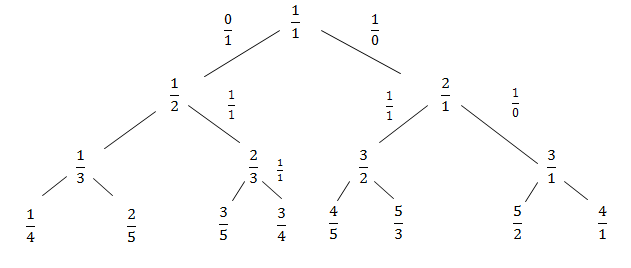
\includegraphics[scale=.75]{Stern.png}
\end{center}
\centerline{\vdots}

\centerline{Figure.1  Stern-Brocot tree}
\bigskip

One can write a statement, its proof and end sign of the proof as follows:

\begin{fact}
Let $I=\mathbb{R^+}\cup \{\infty, 0 \}. $  If the map $\eta: I \rightarrow [0,1], $ is defined by
$$ \eta (x) = \frac{x}{x+1}, \ x \in \mathbb{R}^+ , \ \ 
\eta(\infty) = 1 . $$

\begin{proof}  It suffices to prove that $\eta(x) + \eta (x')=\eta (x + x')$. To show this, let $x = \frac{p}{q}$ and $x^\prime = \frac{r}{s}$, then, 

\begin{center}
$\eta(x) + \eta (x') = \frac{\frac{p}{q}}{\frac{p}{q}+1} + \frac{\frac{r}{s}}{\frac{r}{s}+1} = \frac{\frac{p}{q}}{\frac{p+q}{q}} + \frac{\frac{r}{s}}{\frac{r+s}{s}} = \frac{p}{p+q}$ $\oplus$ $\frac{r}{r+s} = \frac{p+r}{p+q+r+s} . $
\end{center}

\begin{center}
$\eta (x + x') = \eta (\frac{p}{q} + \frac{r}{s})= \eta (\frac{p+r}{q+s}) = \frac{\frac{p+q}{r+s}}{\frac{p+q}{r+s}+1} = \frac{\frac{p+q}{r+s}}{\frac{p+q+r+s}{r+s}} = \frac{p+q}{p+q+r+s}.$
\end{center}
Therefore, $\eta (x) + \eta (x')=\eta (x + x')$.
\end{proof}
\end{fact}
\medskip

\noindent{\bf Remark.}  As it is seen in Fact.1 one should not forget to end a proof without the sign that indicates that it's the case.  For, you cal also use the command: \qed 
\medskip

One can also use a different command to write a formula in display mode as:

\begin{exa}  Notice that $\frac{3}{2}, \frac{11}{9}
\in \mathcal{T} \setminus \mathcal{F}.  $  Then
$$\aligned & \eta(x)= \frac{\frac{3}{2}}{\frac{3}{2}+1} = \frac{\frac{3}{2}}{\frac{5}{2}} = \frac{6}{10} = \frac{3}{5} \in \mathcal{F}, \ \text{and} \\
& \eta(x)= \frac{\frac{11}{9}}{\frac{11}{9}+1} = \frac{\frac{11}{9}}{\frac{20}{9}} = \frac{99}{180} = \frac{11}{20} \in \mathcal{F}.
\endaligned $$
\end{exa}
\medskip

You can write definitions as:

\begin{defi} The {\it mediant} of $\frac{p}{q}$ and $\frac{p'}{q'}$ is defined as $\frac{p+{p}'}{q+{q}'} $ and need not be in the lowest terms.
\end{defi}
\medskip

You can also write definitions as:

\noindent{\bf Definition.} The {\it mediant} of $\frac{p}{q}$ and $\frac{p'}{q'}$ is defined as $\frac{p+{p}'}{q+{q}'} $ and need not be in the lowest terms.
\medskip

You can give citations within the article by using the command \cite{Bonanno} \cite{Apostol} \cite{Barnsley} \cite{Davidson} \cite{Devaney}
\cite{Elaydi}.

\bigskip

\centerline{\bf 3. Continuing with Additional Sections.} 

Typically a paper begins with an Abstract, Introduction, a section where basic tools and techniques are introduced, and subsequent sections where the subject is developed.
\medskip

\begin{defi} A code that corrects all error patterns of weight at most $t$ and does not correct any error pattern of weight $t+1$ is called a {\it t error-correcting code}.
\end{defi}
\medskip

\begin{exa} Given $C=\{000, 010, 101, 111\}$. $C$ has distance 3 so by theorem 1.2, $C$ detects all error patterns of weight 1 or 2, but does not detect error patterns of weight 3. Hence, $C$ is a 2 error-correcting code.
\end{exa}

\medskip

\begin{defi}  Any expression of the form
$$x = a_{0} + \cfrac{1}{a_{1}+\cfrac{1}{a_{2}+\cfrac{1}{\ddots+\cfrac{1}{a_{n}+\cfrac{1}{\ddots}}}}}$$
is called an {\bf infinite continued fraction} will be denoted by $[a_0; a_1, a_2, \dots ] .$ 
\end{defi}
\medskip

\begin{exa}
Let $x$ be the Golden Ratio $\frac{1+\sqrt{5}}{2}\approx\:\frac{3.236}{2}, $ then we observe that
\begin{center}
3.236 = $\mathbf{1}\cdot$2 + 1.236\\
2 = $\mathbf{1}\cdot$1.236 + 0.764\\
1.236 = $\mathbf{1}\cdot$0.764 + 0.472\\
0.764 = $\mathbf{1}\cdot$0.472 + 0.292 .\\
$\vdots$
\end{center}

Therefore, $\frac{1+\sqrt{5}}{2}$=[1;1,1,1,$\cdots$] which can be proved by letting

\begin{center}
 $ x = 1 + \cfrac{1}{1
          + \cfrac{1}{1
          + \cfrac{1}{1 + \cfrac{1}{\ddots} } } },$
\end{center}
which is the continued fraction generated by [1;1,1,1,$\cdots$].
The continued fraction above can also be written as 
$x = 1 + \frac{1}{x} , $ since the 1's are infinite, and this implies that $ x^2 - x - 1 = 0 . $  
Therefore the continued fraction would have to equal the positive solution to this polynomial, which is $\frac{1+\sqrt{5}}{2}$ by the quadratic formula.  Recall that this is the classical definition of the Golden Ratio.
\end{exa}

\medskip

Now, having continued fraction defined, we will explore some of its basic properties.
\medskip

\begin{prop}  For any finite continued fraction we have
$$[a_{0};a_{1},\dots,a_{n}] = \left\{\begin{matrix}
[a_{0};a_{1},\dots,a_{n-1}+1]\: if\: a_n = 1\\
[a_{0};a_{1},\dots,a_{n}-1,1]\: if\: a_n \neq 1
\end{matrix}\right.$$

\begin{proof}  If $a_n$ = 1, then
\begin{center}
$a_0 + \cfrac{1}{a_1
          + \cfrac{1}{a_2
          + \cfrac{1}{\ddots \cfrac{1}{a_{n-1} + \cfrac{1}{1}} } } }$ = $a_0 + \cfrac{1}{a_1
          + \cfrac{1}{a_2
          + \cfrac{1}{\ddots \cfrac{1}{a_{n-1} + 1} } } }, $ since $\frac{1}{1}=1. $
\end{center}
Therefore, $[a_{0};a_{1},\dots,a_{n-1},1]$ = $[a_{0};a_{1},\dots,a_{n-1} + 1].$  Similarly, if $a_n$ $\neq$ 1, then
\begin{center}
$a_0 + \cfrac{1}{a_1
          + \cfrac{1}{a_2
          + \cfrac{1}{\ddots \cfrac{1}{a_{n}} } } }$ = $a_0 + \cfrac{1}{a_1
          + \cfrac{1}{a_2
          + \cfrac{1}{\ddots \cfrac{1}{(a_{n}-1) + 1} } } }$\\ = $a_0 + \cfrac{1}{a_1
          + \cfrac{1}{a_2
          + \cfrac{1}{\ddots \cfrac{1}{a_{n} - 1 + \cfrac{1}{1}} } } }.$
\end{center}

\noindent Therefore,  $[a_{0};a_{1},\dots,a_{n}]$ = $[a_{0};a_{1},\dots,a_{n} - 1,1]$ if $a_n \neq 1. $
\end{proof}
\end{prop}
\medskip

\begin{thm}   For any $x\in \mathbb R, $ there exists a unique continued fraction
$[a_0, a_1, a_2, \dots ] $ such that 
$$ x=[a_0, a_1, a_2, \dots ] . $$
Furthermore, this continued fraction is finite if $x\in \mathbb Q. $

\begin{proof}
 Since the assertion is trivial if $x$ is an integer, we will assume that $x$ is not an integer.  Let $a_0 $ be the greatest integer less than or equal to $x. $  Then, $x=a_0 + \frac{1}{r_1}. $  Since $\frac{1}{r_1}=x-a_0 <1, \ r_1 $ is not an integer and $r_1>1. $  In general, if
$r_n $ is not an integer, let $a_n $ be the greatest integer less than or equal to $r_n ,$ and
define $r_{n}=a_n-\frac{1}{r_{n+1}}. $  Then $r_{n+1} >1. $  This process continues as long as $r_n$'s are not integers.  Now, from $x=a_0 + \frac{1}{r_1}, $ we have $x=[a_0; r_1], $ and in general,
$r_{n}=a_n-\frac{1}{r_{n+1}} $ implies that
$$ x=[a_0; a_1, a_2, \dots , a_{n-1}, r_n], \ n\geq 1, $$
provided that $r_1, r_2, \dots , r_n $ are not integers. 

Now, if $x $ is a rational number, then each $r_n $ is also a rational number.  If $r_n=\frac{a}{b} $ form some $a,b \in \mathbb Z, $ then $r_n - a_n =\frac{a-b a_n}{b}=\frac{c}{b}, $ where $c<b $ since
$r_n -a_n <1. $  If $c=0, $ i.e., $a_n $ is an integer, then $r_n $ is an integer and we are done.  
If $c\neq 0, $ then $r_{n}=a_n-\frac{1}{r_{n+1}}$ implies that $r_{n+1}=\frac{b}{c}, $ and hence, $r_{n+1}$ has smaller denominator than that of $r_n. $  Hence, continuing in this manner, eventually we will reach $a_m=r_m $ for some $m. $  This fact, together with the representation
$ x=[a_0; a_1, a_2, \dots , a_{n-1}, r_n], $ imply that $x$ has a finite continued fraction representation.

If $x$ is irrational, then all $r_n$'s are irrational, and hence, the process above continues indefinitely.  Letting $[a_0; a_1, \dots , a_n]=\frac{p_n}{q_n}, $ we have 
$x=[a_0; a_1 \dots, a_{n-1}, r_n]. $  By Fact 3, 
$$ x=\frac{p_{n-1}r_n + +p_{n-2}}{q_{n-1}r_n +q_{n-2}}, \ \ n\geq 2. $$
Since $\frac{p_n}{q_n} =\frac{p_{n-1}a_n + +p_{n-2}}{q_{n-1}a_n +q_{n-2}}, $ we have
$$ \aligned \left | x - \frac{p_n}{q_n} \right | & =
\left |\frac{(p_{n-1}q_{n -2} - q_{n-1} p_{n-2}) (r_n-a_n)}{(q_{n-1}r_n+q_{n-2})(q_{n-1} a_n+q_{n-2})}
\right | \\
& < \frac{1}{|(q_{n-1}r_n+q_{n-2})(q_{n-1} a_n+q_{n-2})|}< \frac{1}{q_n^2}, \endaligned $$
since $|r_n-a_n|<1 $ and $|p_{n-1}q_{n -2} - q_{n-1} p_{n-2}|<1 $ be Fact 4.  Hence, it follows from Fact 7 that
$\lim_n \frac{p_n}{q_n}=x.$

It remains to prove the uniqueness of the representation.  Assume that 
$$[a_0; a_1, a_2, \dots ]=x=[a'_0; a'_1, a'_2, \dots ]. $$
Obviously, $a_0=a'_0=$greatest integer less than or equal to $x. $  If $a_i=a'_i $ for $1\leq i \leq k,$
then $p_i=p'_i $ and $q_i=q'_i $ for $1\leq i \leq k. $  Thus, 
$$ x=\frac{p_n r_{n+1}+p_{n-1}}{q_n r_{n+1}+q_{n-1}}
=\frac{p'_n r'_{n+1}+p'_{n-1}}{q'_n r'_{n+1}+q'_{n-1}}
=\frac{p_n r'_{n+1}+p_{n-1}}{q_n r'_{n+1}+q_{n-1}}, $$
which implies that $r_{n+1}=r'_{n+1}. $  Since 
$a_{n+1}=$greatest integer less than or equal to $r_{n+1}$ and 
$a'_{n+1}=$greatest integer less than or equal to $r'_{n+1}, $ we obtain that
$a_{n+1}=a'_{n+1} $ by induction. 
\end{proof}
\end{thm}
\medskip

\noindent{\bf Remark.}  From Theorem above, we deduce that a rational number $x$ has a a finite continued fraction while an irrational number has an infinite sequence continued fraction representation.
\medskip

\noindent{\textbf{Definition}}: The sum in LaTeX is written as 
$\sum\limits_{n=0}^\infty a_{n}$.

\bigskip

\centerline{\bf 4. Matrix Representation and Coding.}
\medskip

There is a 1-1 correspondence between the elements in the $\mathbb Q^{+} $ and elements of the set of $2 \times 2$ matrices with integer entries $SL(2, \mathbb Z)$. This correspondence is very instrumental in studying the dynamics on continued fractions.
\medskip

We can describe each rational number as a matrix of the parent fractions \cite{Barnsley},

\begin{center}
$x=\cfrac{p}{q} + \cfrac{{p}'}{{q}'}\equiv\begin{pmatrix}
p &p' \\ 
q &q' 
\end{pmatrix}$
\end{center}

This association defines a function $\Phi : \mathcal{F} \to SL(2, \mathbb Z) $ by
$$\Phi (\frac{p}{q} + \frac{{p}'}{{q}'})= 
\begin{pmatrix} p & p' \\  q & q'  \end{pmatrix}. $$

\medskip

\begin{exa}
$\Phi (\cfrac{9}{11} )= \Phi (\cfrac{5}{6} + \cfrac{4}{5} ) =  \begin{pmatrix}
5 &4 \\ 
6 &5 
\end{pmatrix}. $
\end{exa}
\medskip

This matrix representation has the following property.  Let 
$$\cfrac{{1}}{{2}}=\begin{pmatrix}
1 &0 \\ 
1 &1 
\end{pmatrix}=:L \ \ \text{and}  \ \ \cfrac{{2}}{{1}}=\begin{pmatrix}
1 &1 \\ 
0 &1 
\end{pmatrix}=:R . $$

Then it follows that 

\begin{fact}
$\begin{pmatrix}
1 &0 \\ 
k &1 
\end{pmatrix}=:L^{k} , $ and 
$\ \begin{pmatrix}
1 &k \\ 
0 &1 
\end{pmatrix}=:R^{k}. $

\begin{proof}  Trivial.
\end{proof}
\end{fact}
\medskip

\begin{thm} \cite{Devaney} \cite{Elaydi} \cite{Apostol} Let $H$ be a parity-check matrix for a linear code $C$. Then $C$ has distance $d$ iff any set of $d-1$ rows of $H$ are linearly independent and at least one set of $d$ rows of $H$ is linearly dependent.
\end{thm}

\begin{proof} If $G$ is a generator matrix for $C$, place $G$ in RREF. Rearrange the columns of the RREF so that the leading columns come first and form an identity matrix. The result is a matrix $G^\prime$ in standard form which is a generator matrix for a code $C^\prime$ equivalent to $C$.
\end{proof}
\medskip

Having the infinite string coding of any real number in $\{L,R\}^{\mathbb N}$ defined, we can exploit some structural properties of 
$\{L,R\}^{\mathbb N}$ to study its deeper features.

\bigskip



\bibliographystyle{amsplain}
\bibliography{capstone}


\end{document}



